\documentclass{beamer}

% For more themes, color themes and font themes, see:
% http://deic.uab.es/~iblanes/beamer_gallery/index_by_theme.html
%
\mode<presentation>
{
  \usetheme{Madrid}       % or try default, Darmstadt, Warsaw, ...
  \usecolortheme{beaver} % or try albatross, beaver, crane, ...
  \usefonttheme{serif}    % or try default, structurebold, ...
  \setbeamertemplate{navigation symbols}{}
  \setbeamertemplate{caption}[numbered]
} 

\usepackage{tikz}
\usetikzlibrary{decorations.markings,angles}
\usepackage{tikz-3dplot} 

\usepackage{amsmath}


\begin{document}

\title[3d]  
{Two-fluid simulations of waves and reconnection with Mancha code}
\author[]{Beatrice Popescu Braileanu }
\institute[]{PhD advisors: \and \'Angel de Vicente \and %
                      Elena Khomenko}
\date{September 1, 2016}

\begin{frame}
\maketitle
\end{frame}

\begin{frame}[t]{Sun atmosphere layers}
\vspace*{-22pt}
\begin{columns}[b]
    \begin{column}{0.6\textwidth}
		Photosphere
        \begin{itemize}
					\item collisions dominated: LTE, MHD 
					\item	relatively easy observations 
					\item	diagnostics techniques well developed 
        \end{itemize}
    \end{column}
    \begin{column}{0.5\textwidth}
       % \rule{\textwidth}{0.75\textwidth}
			\begin{figure}[t]
			 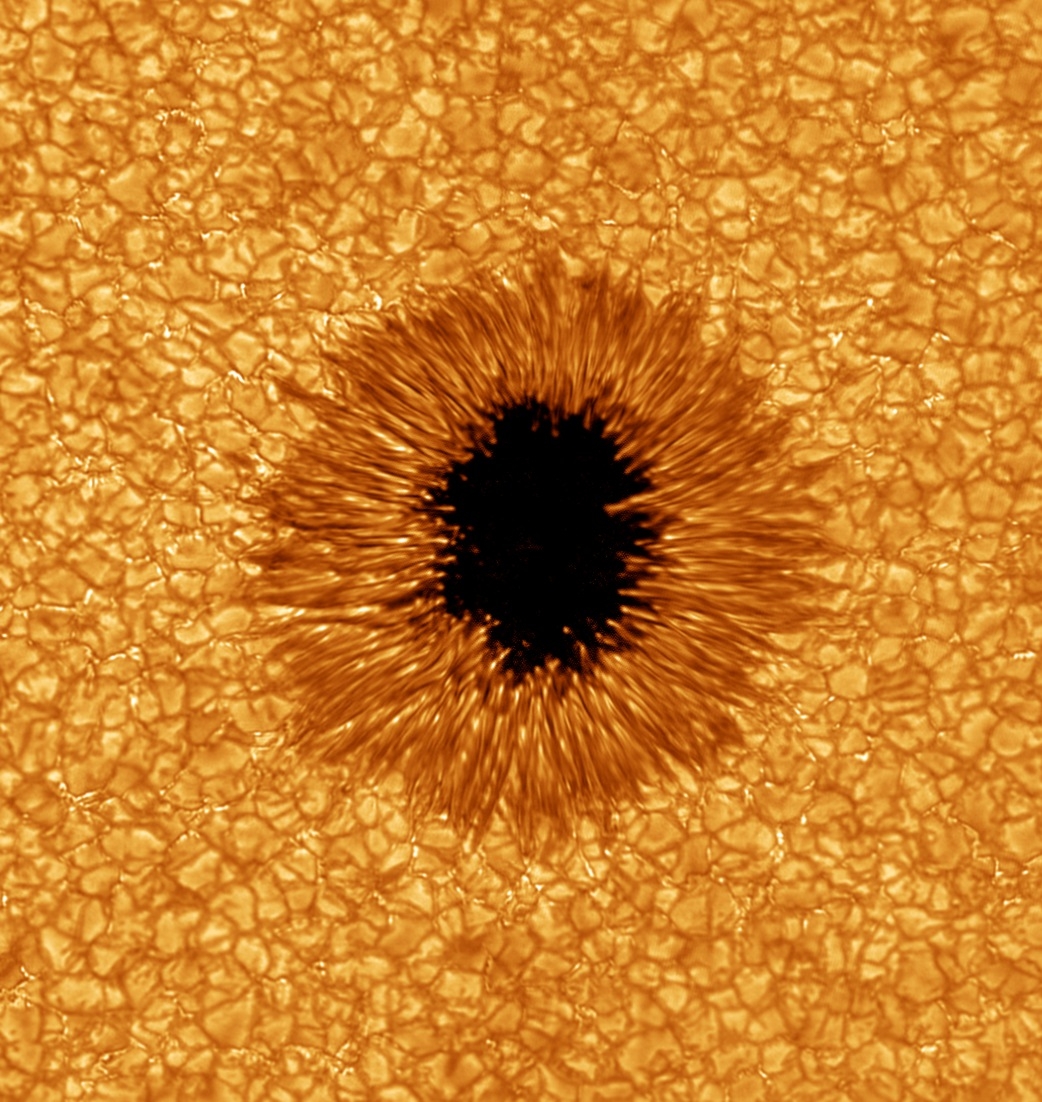
\includegraphics[scale=0.08]{phot.jpg}
			\end{figure}
    \end{column}
\end{columns}

\begin{columns}[b]
    \begin{column}{0.6\textwidth}
		Chromosphere
        \begin{itemize}
					\item not fully collisionally coupled: NLTE, No MHD (frequently not taken into account)
					\item very few spectral lines 
					\item complicated radiative diagostics 
        \end{itemize}
    \end{column}
    \begin{column}{0.5\textwidth}
       % \rule{\textwidth}{0.75\textwidth}
			\begin{figure}[t]
			 \centering
			 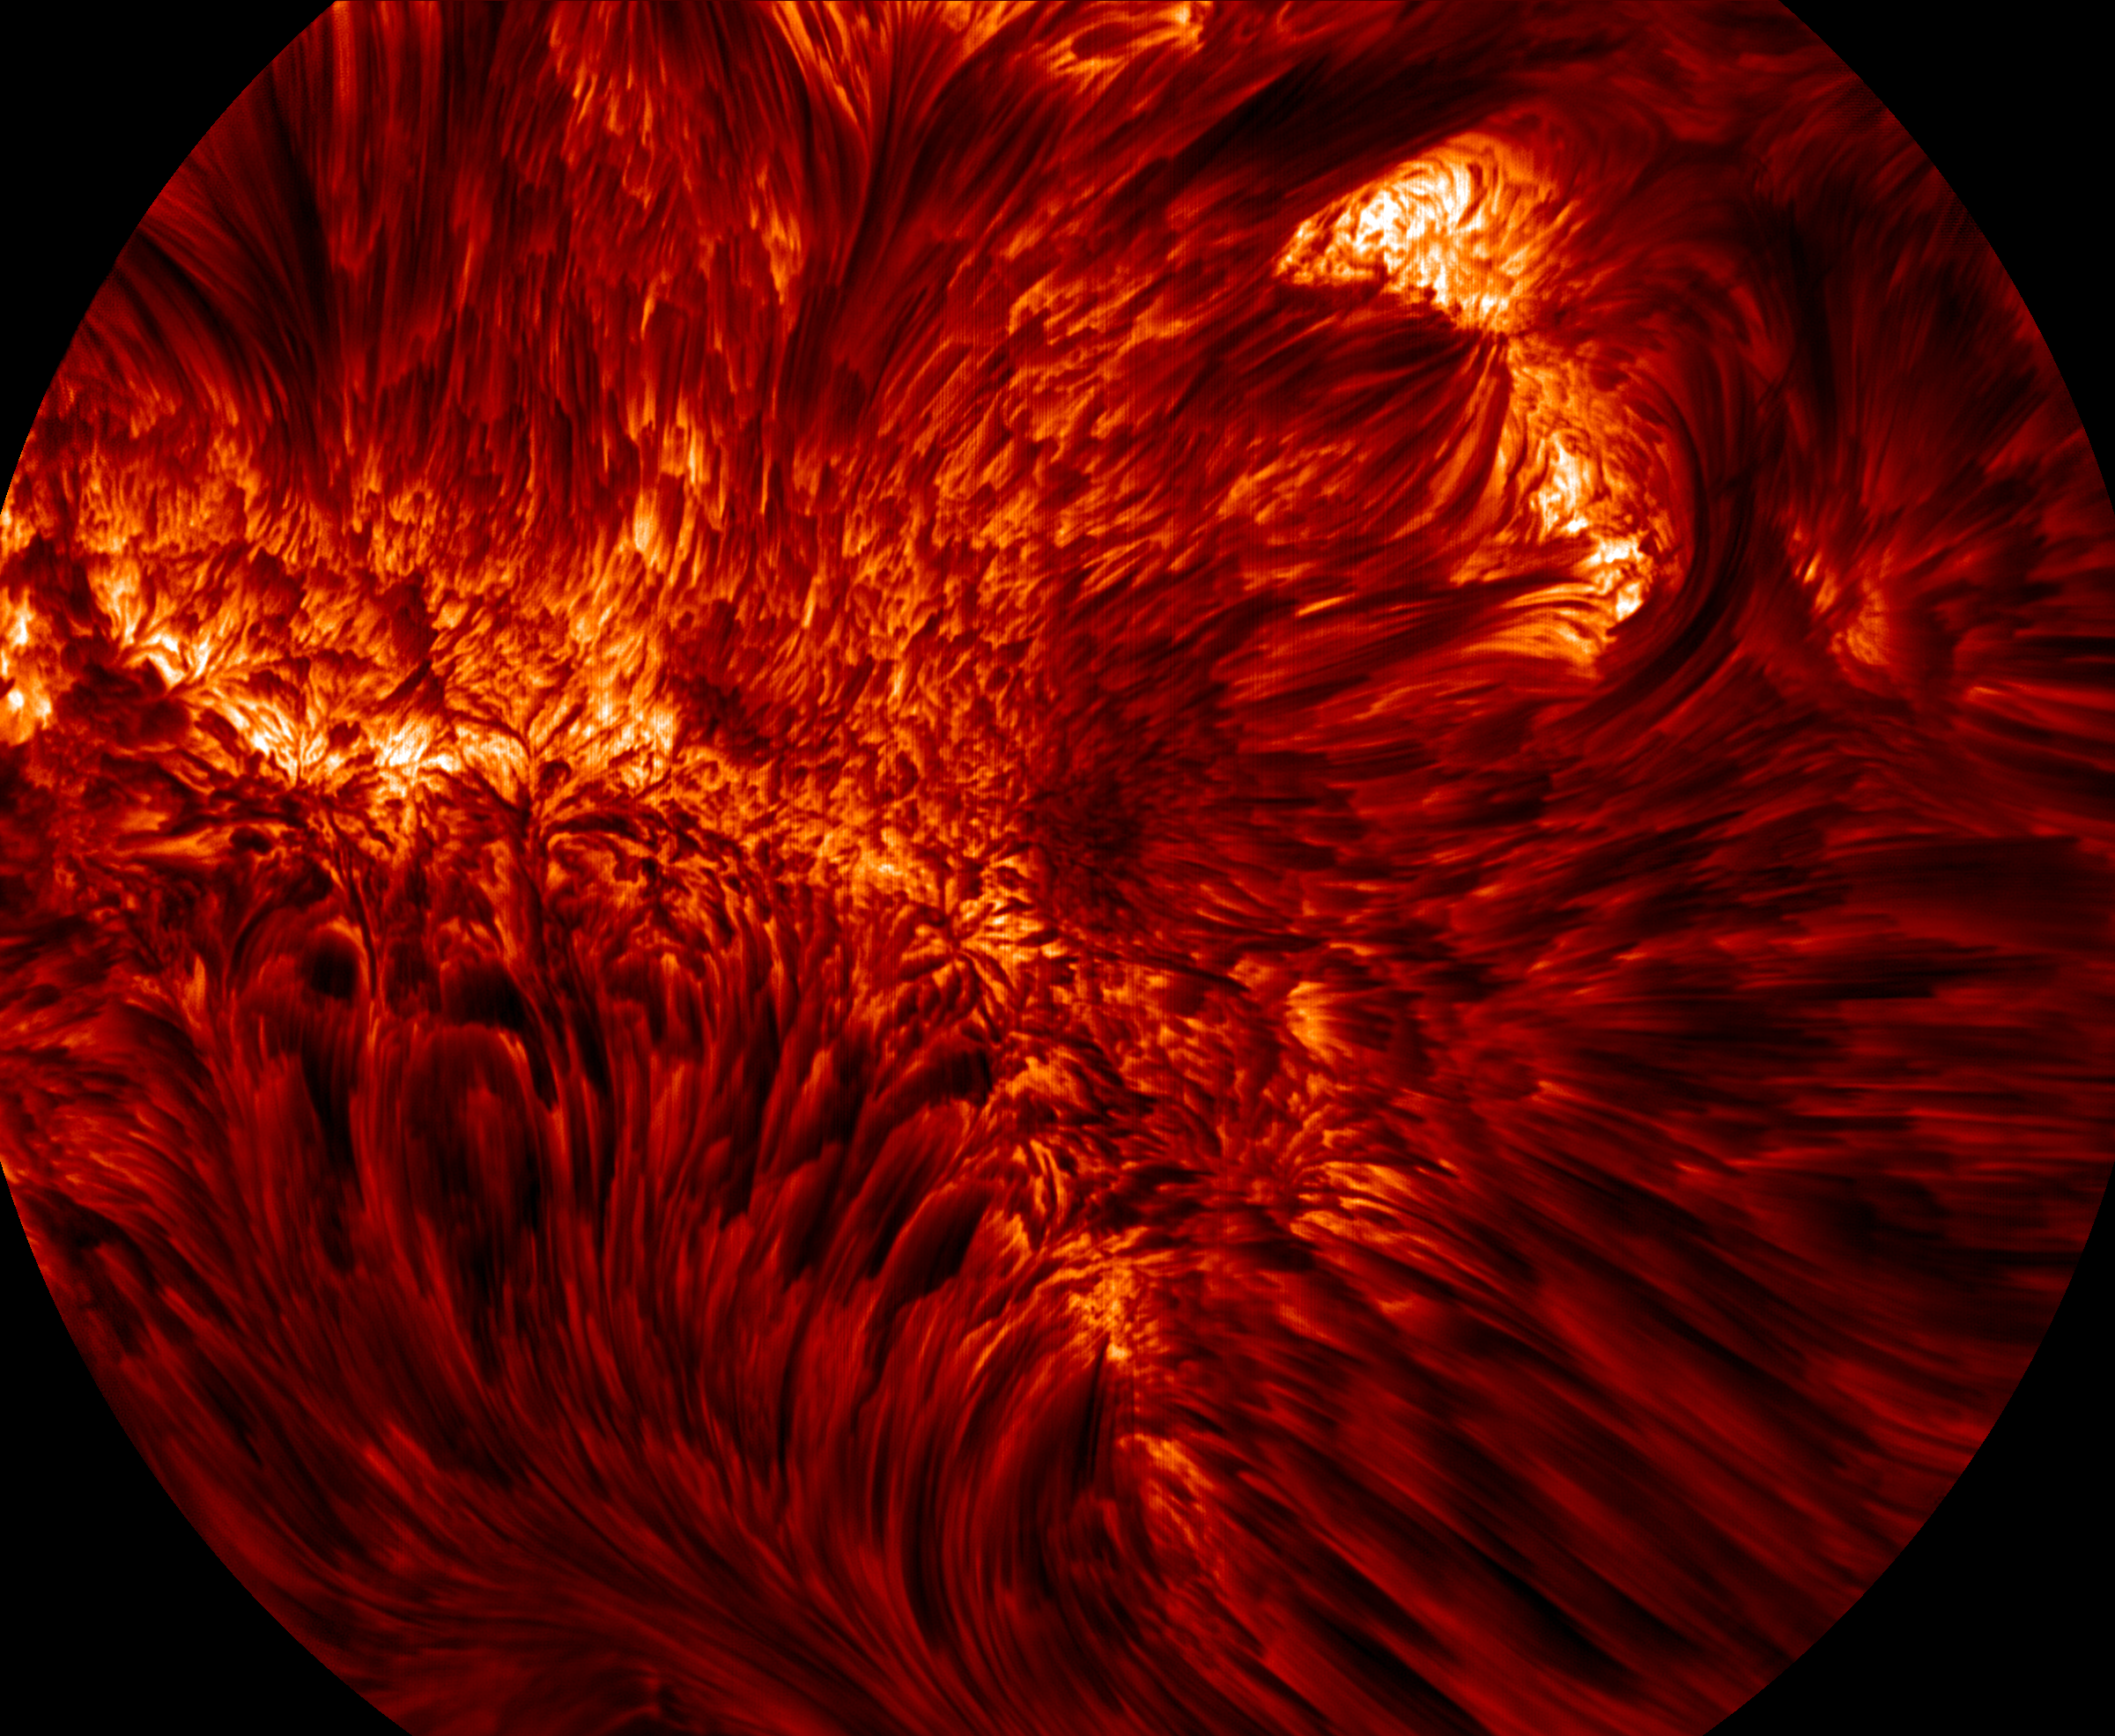
\includegraphics[scale=0.03]{chrom.png}
			\end{figure}
    \end{column}
\end{columns}

\begin{columns}[c]
    \begin{column}{0.6\textwidth}
		Corona
        \begin{itemize}
					\item magnetically dominated 
					\item very low density
					\item all ionized, MHD can be applied
        \end{itemize}
    \end{column}
    \begin{column}{0.5\textwidth}
			\begin{figure}[t]
			 \centering
			 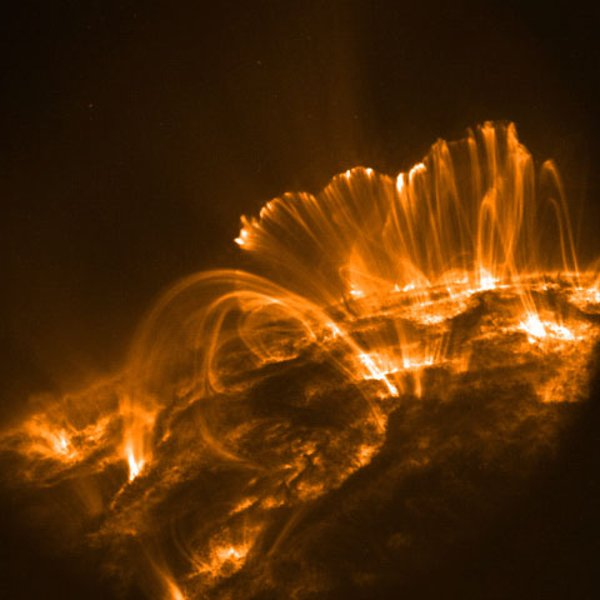
\includegraphics[scale=0.11]{corona.jpg}
			\end{figure}
    \end{column}
\end{columns}

\end{frame}

\begin{frame}{2 fluids model}
\begin{itemize}
\item 13 partial differential equations: 10 variables p , $\rho$ and v of the 2 fluids: charges(\_c) and neutrals(\_n) + magnetic field
\item hydrostatic equilibrium(\_0 : $p_c0, p_n0, \rho_c0, \rho_n0$, B), $v_{c0}=v_{n0}=0$
 
\begin{itemize}
\item charges:
\begin{equation}
\rho_{c0}\vec{g} - \vec{\nabla} p_{c0} + \frac{1}{\mu_0} (\nabla \times \vec{B_0}) \times \vec{B_0} = 0
\end{equation}

\item neutrals:
\begin{equation}
\rho_{n0}\vec{g} - \vec{\nabla} p_{n0}  = 0
\end{equation}

\end{itemize}
\item perturbation(\_1 for the 13 variables)

\item total variables  $x = x_0 + x_1$ for x = $p_c,p_n, \rho_c, \rho_n, B$, $v_c = v_{c1},v_n = v_{n1}$
\end{itemize}

\end{frame}

\end{document}
